\section*{5/6}
  $$
    \phi(s)= \phi_{X_1}(s) = \sum_{k = 0}^{\infty} P_k s^k
  $$
  $$
    \pi_0  = P(\text{ branching process ever dies out}) = \lim_{n \to \infty}d_n
  $$
  \underline{Note}: $d_n$ is an incrasing sequence
  \subsection*{Properties of $\phi$}
    \begin{enumerate}
      \item $\phi(0) = P_0 > 0$
      \item $\phi(1) = 1$ because $\phi(1) = \sum_{k = 0}^{\infty}P_k = 1$
      \item 
      $$
        \phi'(s) = \sum_{k = 0}^{\infty}kP_k s^{k - 1} \ge 0
      $$
      Therefore, $\phi$ is increasing
      \item
      $$
        \phi"(s) = \sum_{k = 1}^{\infty}k(k-1)P_k s^{k-2} \ge 0
      $$
      Therefore, $\phi$ is convex
    \end{enumerate}
  \subsection*{two cases of geometry of $\phi$}
    \begin{enumerate}
      \item $\phi$ is always above the diagonal, $\pi_0 = \lim_{n \to \infty}
        d_n = 1$. We can tell if this is the case for $\phi$ if the 
        $\phi'(1) < 1$.
      \item $\phi$ is not always above the diagonal. In this case, $\pi_0 = 
        \lim_{n \to \infty} d_n$, $d_n$ converges to the smallest solution to 
        $s = \phi(s)$. We can tell if this is the case for $\phi$ if the i
        $\phi'(1) > 1$.
    \end{enumerate}
    To calculate $\phi'(1)$, we just do $\sum_{k = 1}^{\infty} kP_k = \mu$.\\
    In summary,
    $$
      \mu = \sum_{k = 1}^{\infty} k P_k
    $$
    If $\mu \le 1$, $\pi_0 = 1$.\\
    If $\mu > 1$, $\phi(s) = sum_{k = 0}^{\infty}P_k s^k$ and find the
      smallest solution to $s = \phi(s)$.\\

    \noindent\underline{Example}: 
    $$
      P_k = p^k(1 - p)
    $$
    \underline{Note}: Not geometric. It's more like geometric - 1 because
      geometric cannot have 0.\\
    $$
      \mu = \frac{1}{1-p} - 1 = \frac{p}{1 - p}
    $$
    If $p \le \frac{1}{2}$, $\pi_0 = 1$.\\
    Suppose that $p > \frac{1}{2}$.Then,
    \begin{eqnarray*}
      \phi(s) & = & \sum_{k = 0}^{\infty}s^k p^k(1 - p)\\
        & = & \frac{1 - p}{1 - ps}\\
        & = & s
    \end{eqnarray*}
    $(ps - 1 + p)(s - 1) = 0$, so $\pi_0 = \frac{1 - p}{p}$.\\

  \noindent\underline{Example}:
    \begin{tabular}{c | c c c c}
      $k$ & 0 & 1 & 2 & 3\\
      $P_k$& $\frac{1}{8}$ & $\frac{3}{8}$ & $\frac{3}{8}$ & $\frac{1}{8}$
    \end{tabular}
    $\mu = \frac{3}{2} > 1$.\\
    $\pi_0 : \phi(s) = \frac{1}{8} + \frac{3}{8}s + \frac{3}{8}s^2 + 
      \frac{1}{8}s^3 = s$\\
    Solving this gets us $s = 1, -\sqrt{5} - 2, \sqrt{5} - 2$.\\
    Take the smallest non-negative solution, which is $\sqrt{5} - 2$.\\

  \subsection*{Limiting probabilities}
    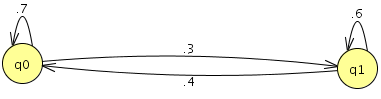
\includegraphics[height=40mm]{5_6.png}
    \begin{eqnarray*}
      P & = & \left[\begin{array}{c c}
        .7 & .3\\
        .4 & .6
      \end{array}\right]\\
      P^4 & = & \left[\begin{array}{c c}
        .5749 & .4251\\
        .5668 & .4332
      \end{array}\right]\\
      P^8 & = & \left[\begin{array}{c c}
        .572 & .428\\
        .570 & .430
      \end{array}\right]\\
    \end{eqnarray*}
    The matrix elements appear to converge and the rows become almost 
    identical. Why?\\
    \begin{definition}
      State $i$ has \underline{period} $d$ if $P^{n}_{ii} > 0$, then $d | n$ and
      $d$ is the largest of such positive integer.
    \end{definition}
    \noindent\underline{Example}: Simple symmetrical random walk on $\mathbb{Z}$.\\
      The period of any state is 2 because you can return to original position 
      if you can walk forth $k$ steps and walk back $k$ steps where $k \ge 1$.\\

    \noindent\underline{Example}: Random walk on a square. Again, $2$ because you
      can walk around the square or walk forth and back.\\

    \noindent\underline{Example}: Random walk on a triangle. 1 because you can
    return in 2 steps (walk out and back) or 3 steps (walk around the triangle).\\ 

  \noindent It can be shown that a period is the same for all states in the same
    class. If a state has period 1, it is called \underline{aperiodic}. If the chain
    is irreducible, we call it aperiodic if all state have period 1.

